\newpage{}

\section{Simulation Analysis}
\label{sec:simulation}
\paragraph{}


\subsection{For $t<0$}

\par The first simulation using ngspice, was an equivalent simulation to the circuit solved theoretical in the first exercise. Notice that an extra voltage source was introduce with only the purpose to server as an ameter, controlling the current for the dependent voltage source. The results are shown in the table \ref{sim1} that will serve to compare with the results obtained.

\begin{table}[H]
  \centering
  \begin{tabular}{|c|c|}
    \hline    
    {\bf Name} & {\bf Value [A or V]} \\ \hline
    @c1[i] & 0.000000e+00\\ \hline
@g1[i] & -2.51245e-04\\ \hline
@r1[i] & -2.40136e-04\\ \hline
@r2[i] & -2.51245e-04\\ \hline
@r3[i] & -1.11090e-05\\ \hline
@r4[i] & 1.216975e-03\\ \hline
@r5[i] & 2.512453e-04\\ \hline
@r6[i] & -9.76838e-04\\ \hline
@r7[i] & -9.76838e-04\\ \hline
n1 & 5.178860e+00\\ \hline
n2 & 4.933049e+00\\ \hline
n3 & 4.408850e+00\\ \hline
n5 & 4.967487e+00\\ \hline
n6 & 5.731699e+00\\ \hline
n7 & -1.99428e+00\\ \hline
n8 & -3.01172e+00\\ \hline
n9 & 0.000000e+00\\ \hline

  \end{tabular}
  \caption{Operating point. A variable preceded by @ is of type {\em current}
    and expressed in Ampere; other variables are of type {\it voltage} and expressed in
    Volt.}
  \label{sim1}
\end{table}

\subsection{For $t=0$}
\paragraph{}
The second simulation is conducted with the goal to determine $I_x$. This is made by setting $v_s$ to 0 and turning the capacitor into a voltage source $V_x$ which imposes the same potencial between n6 and n8 as the capacitor and operating at $t=0$. 

\par The results below are the results obtained in the simulation. This simulation is not only needed as essencial because with $V_x$ and $I_x$ we will be able to determine the natural response of the sistem in the next steps. 

\begin{table}[H]
  \centering
  \begin{tabular}{|c|c|}
    \hline    
    {\bf Name} & {\bf Value [A or V]} \\ \hline
    @g1[i] & 0.000000e+00\\ \hline
@r1[i] & 0.000000e+00\\ \hline
@r2[i] & 0.000000e+00\\ \hline
@r3[i] & 0.000000e+00\\ \hline
@r4[i] & 0.000000e+00\\ \hline
@r5[i] & 2.874522e-03\\ \hline
@r6[i] & 0.000000e+00\\ \hline
@r7[i] & 0.000000e+00\\ \hline
n1 & 0.000000e+00\\ \hline
n2 & 0.000000e+00\\ \hline
n3 & 0.000000e+00\\ \hline
n5 & 0.000000e+00\\ \hline
n6 & 8.743422e+00\\ \hline
n7 & 0.000000e+00\\ \hline
n8 & 0.000000e+00\\ \hline
n9 & 0.000000e+00\\ \hline

  \end{tabular}
  \caption{Operating point. A variable preceded by @ is of type {\em current}
    and expressed in Ampere; other variables are of type {\it voltage} and expressed in
    Volt.}
  \label{sim2}
\end{table}

\newpage{}
\subsection{Natural Solution}
\paragraph{}

\par In the third simulation we use the simulator to perform a transiet analysis. For this some initial conditions were given to the software which then realized the analysis. The graphics shown represent the transient analysis for the node n6 between [0,20]ms.





\begin{figure}[H]
    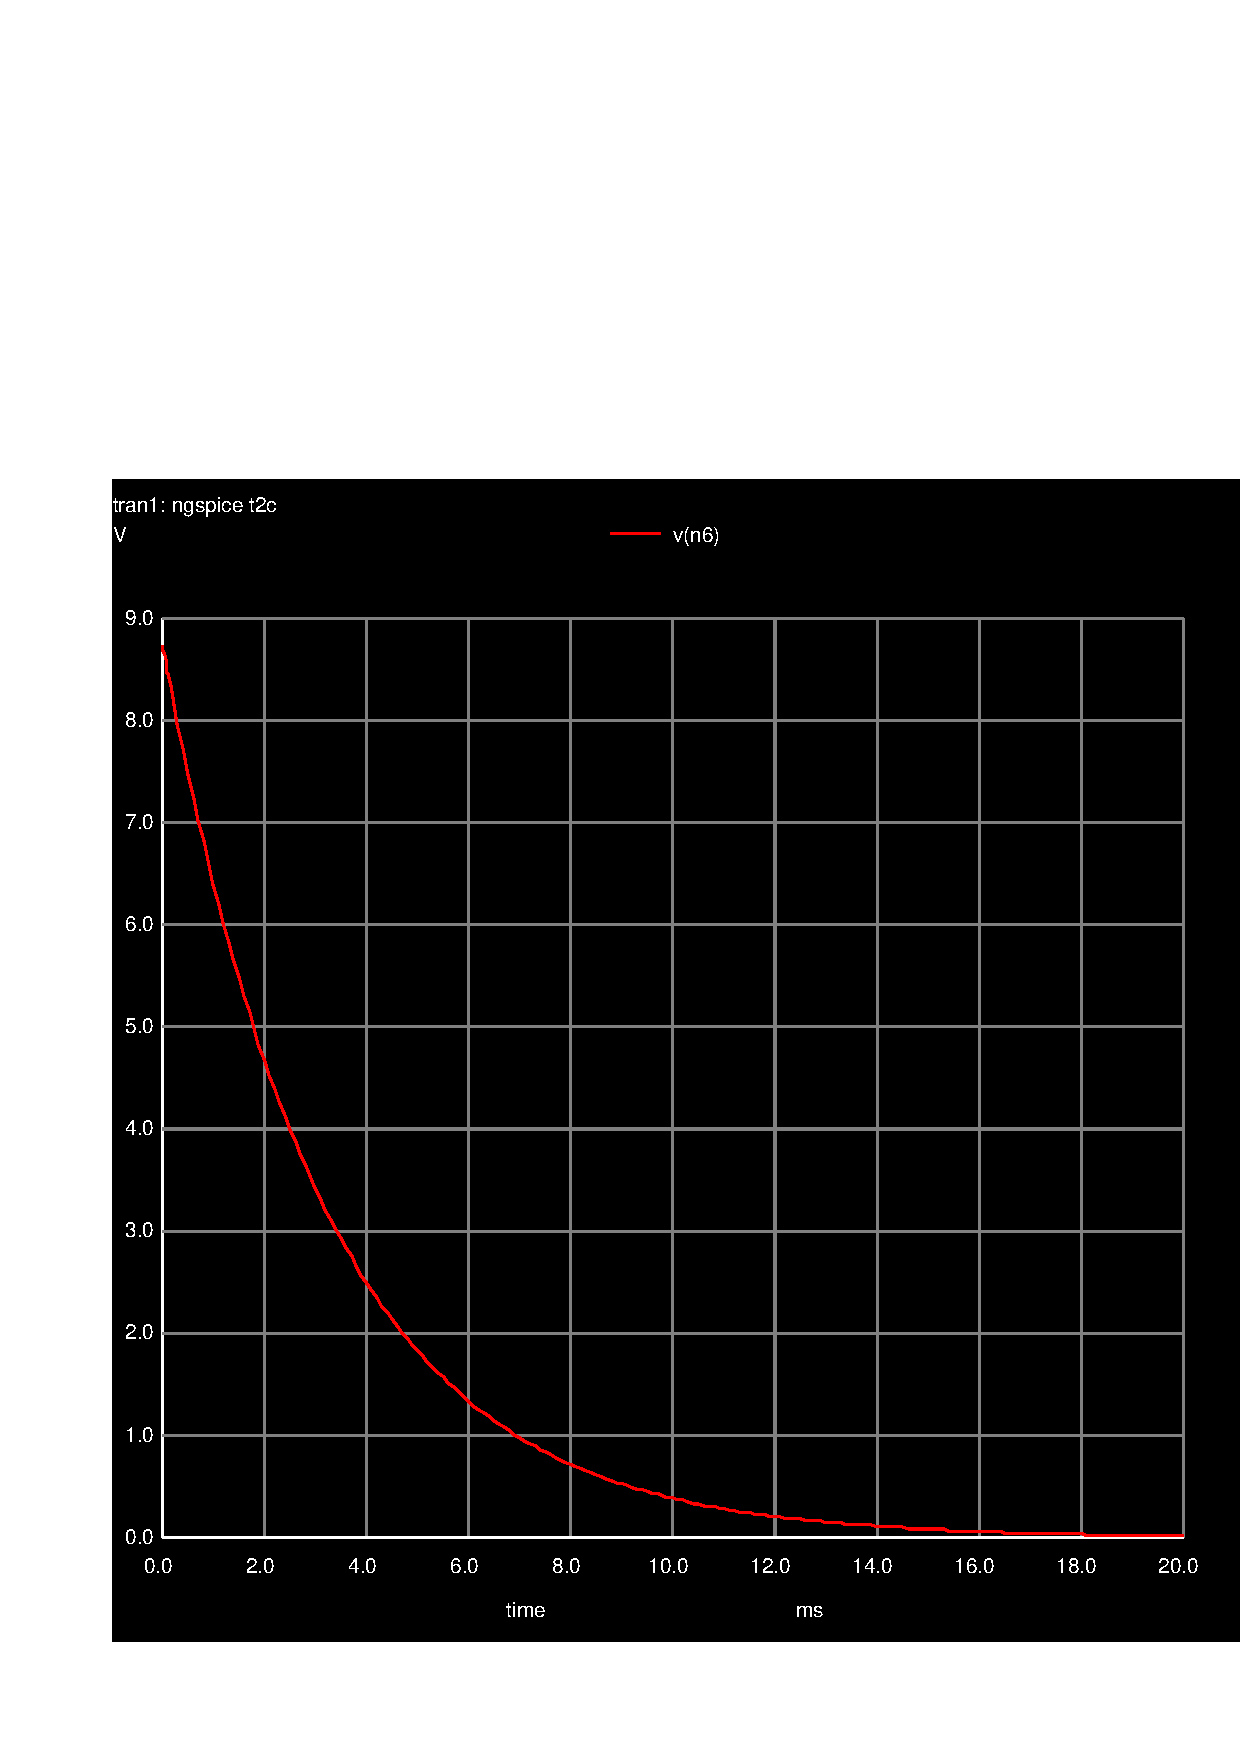
\includegraphics[width=0.4\linewidth]{naturalsim.pdf}
    \centering
    \caption{Natural Solution}
    \label{mag}
\end{figure}



\subsection{Total Solution}
\paragraph{}

\par The simulation conducted next tried to simulate the total response of the node n6. Imposing the conditions given in the exercise, a report showing the response and the stimulus (which was a analysis in n1) is represented in \ref{total}.

\begin{figure}[H]
    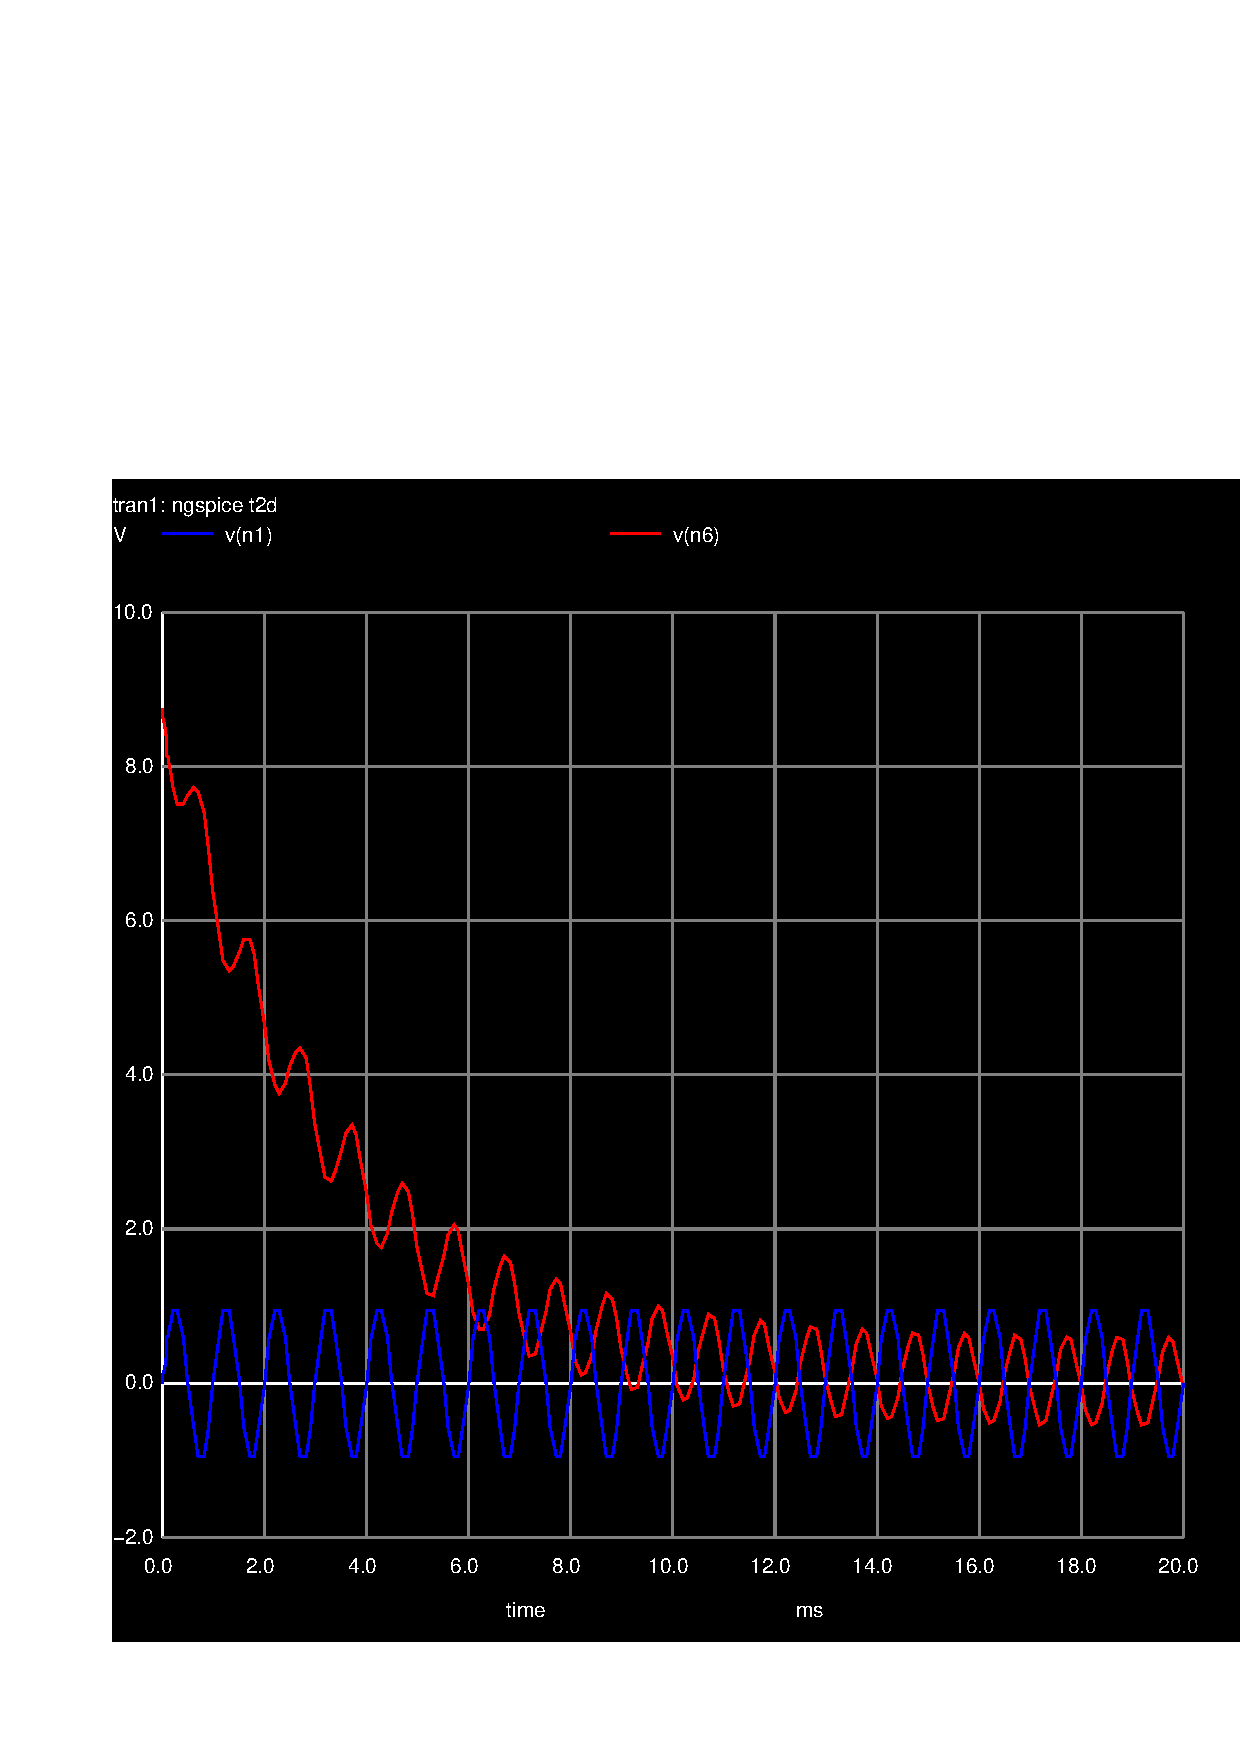
\includegraphics[width=0.4\linewidth]{totalsim.pdf}
    \centering
    \caption{Total Solution}
    \label{total}
\end{figure}

\subsection{Frequency Response}
\paragraph{}

\par At last, a frequency analysis was made in order to compare the frequency response between $v_s$ and n6. The following graphics were obtained.




\begin{figure}[H]
    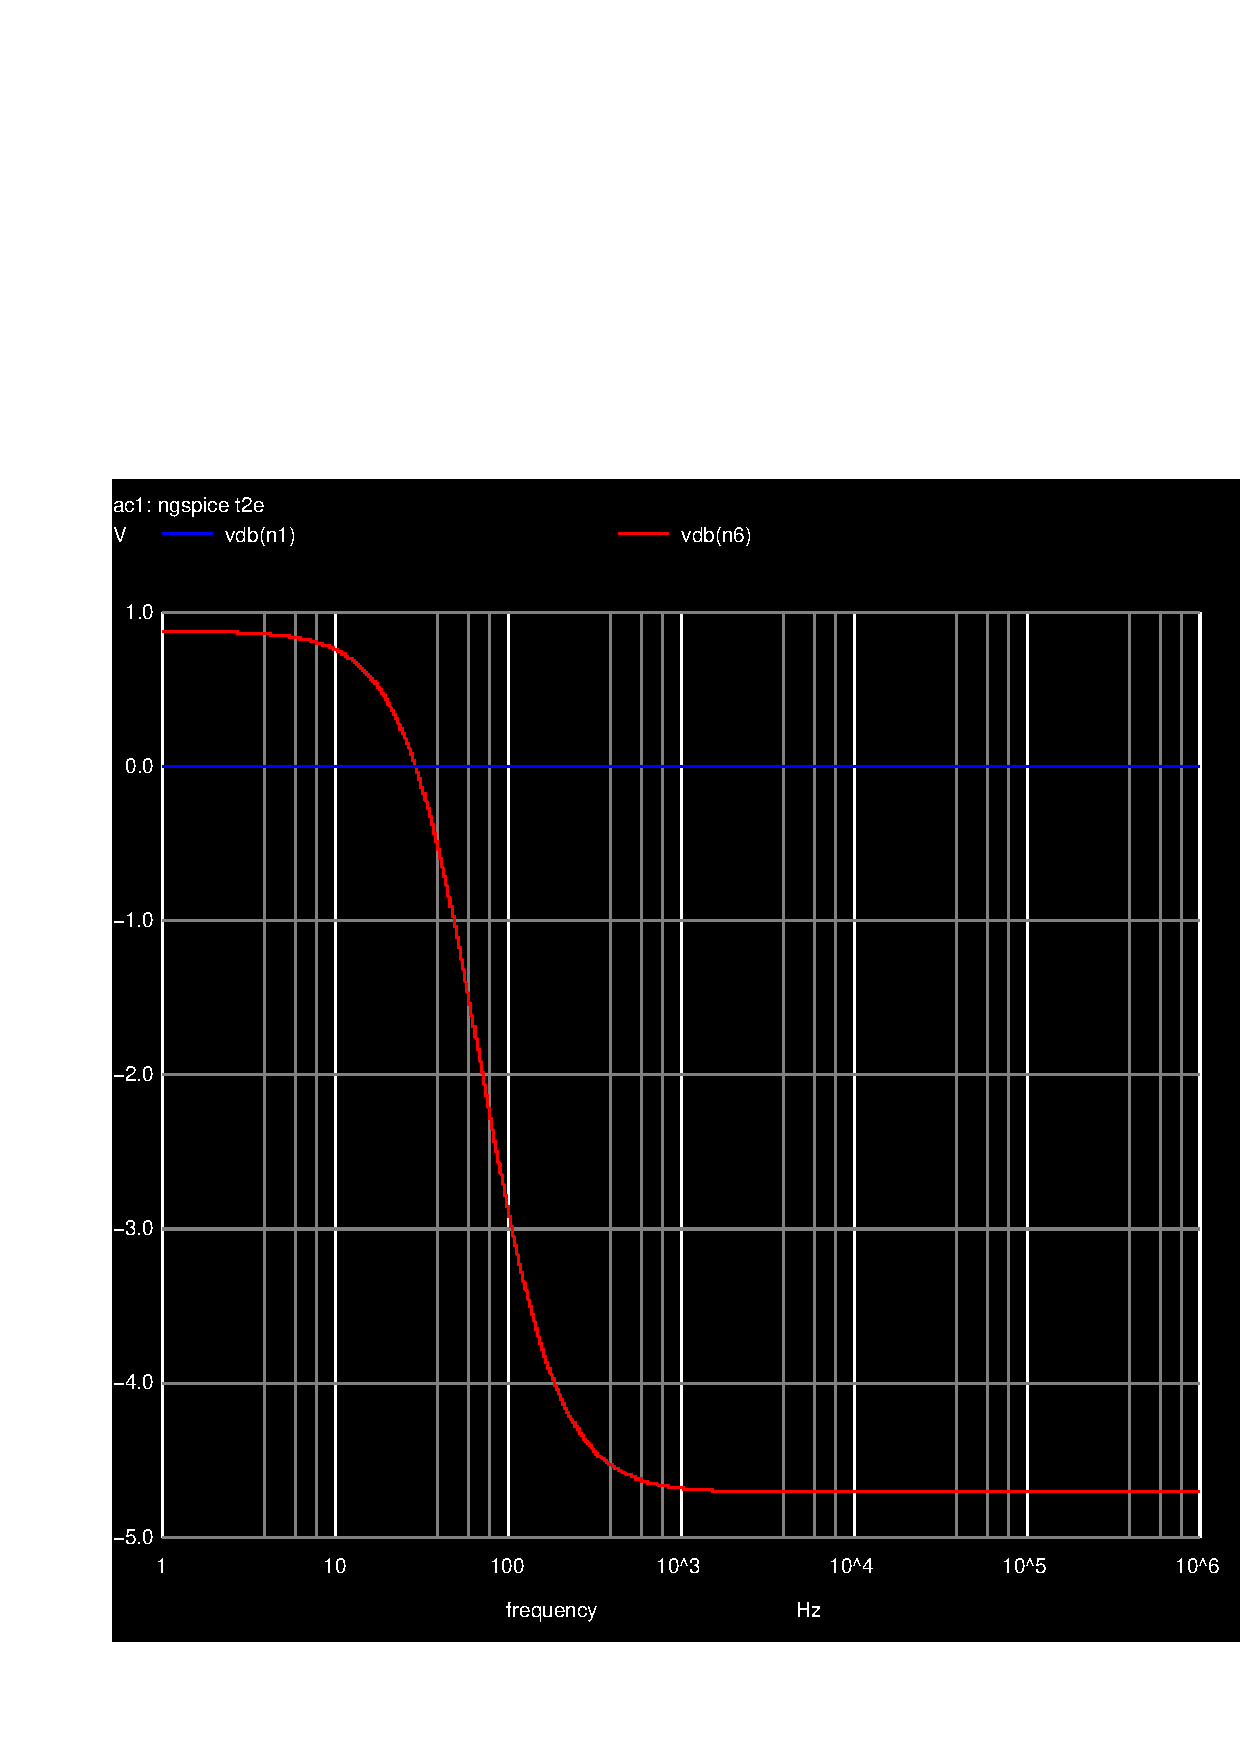
\includegraphics[width=0.4\linewidth]{finalsima.pdf}
    \centering
    \caption{Magnitude}
    \label{mag}
\end{figure}

\begin{figure}[H]
    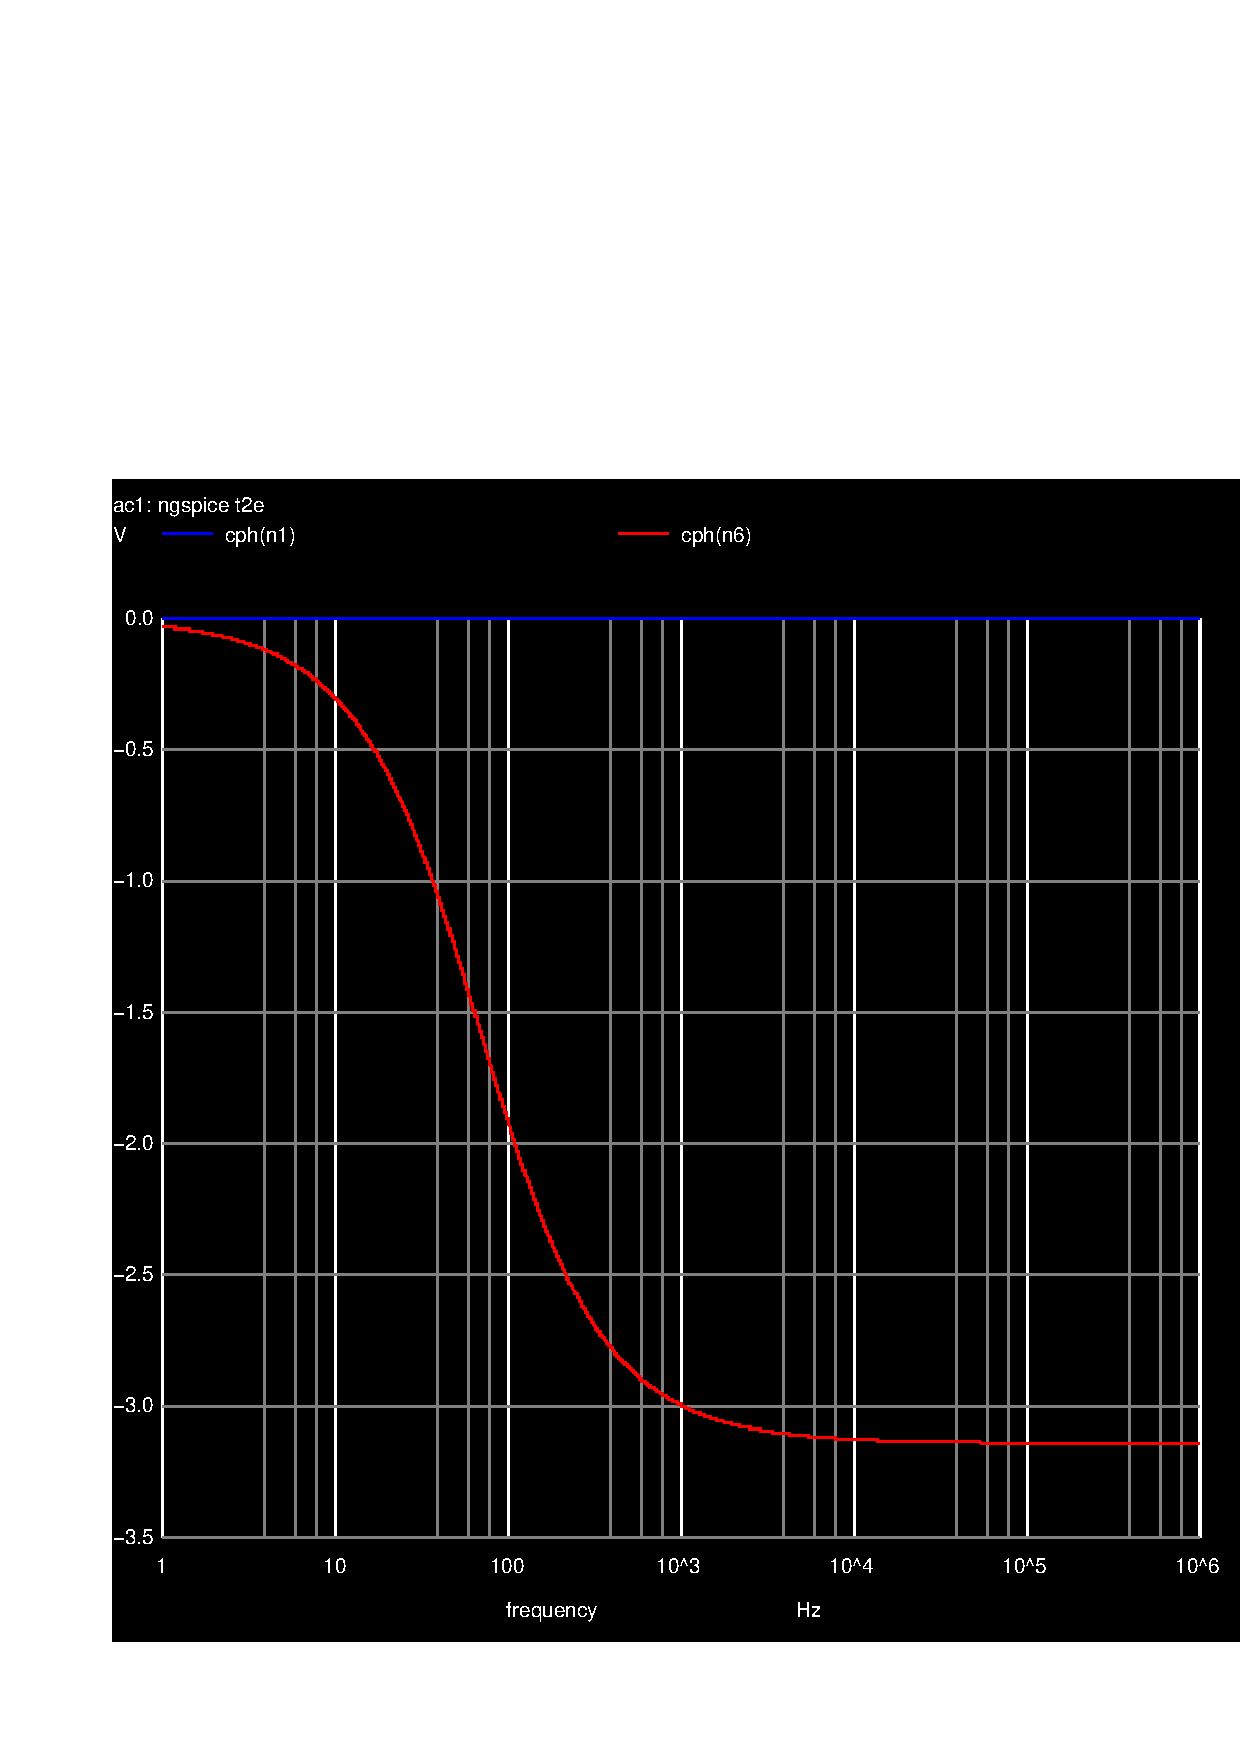
\includegraphics[width=0.4\linewidth]{finalsimb.pdf}
    \centering
    \caption{Phase}
    \label{mag}
\end{figure}

\par We noticed a significant difference bettween them . The frequency response in $V_s$ is null in opposite to the one seen in n6. This is due to the fact that $V_s$ changes ccording to the frequency, thus remaining constant. $V_6$ on the other hand changes its value according to $V_s$ showing a frequency analysis that changes through time.





